\section{Project Management}

To effectively manage time within this project of large nature and short time frame, several project management methodologies and principals were implemented. In order to select the correct approach to incorporate project management into this project, methodologies were chosen based on the projects needs. Time within the project needed to be allocated towards both theoretical and technical research, to select the technologies to be used, models for evaluation and to learn how to use the technologies to implement them. As well as this, time should also be invested into the implementation and training of the models used in this evaluation, this will ensure fair and accurate results, and ample time to perform training. The selected methodology should also allow for flexibility, if issues arise or any risks identified occur, the project can remain on track.

A kanban style approach was the selected project management methodology that met the above needs. The kanban approach is an agile methodology which divides a project into work items, which are then represented on a kanban board, splitting the work items into three categories: to do, in progress and complete. This is used along side its four agile inspired principles: visualise workflow, limit work in progress, focus on flow and continuous improvement. Using this approach means that project members are only ever focused on work in progress, meaning that items in the backlog, or to do section, can be re-prioritised and changed without impacting the project, allowing for continuous improvement of the product. Some benefits of kanban, as reported by \cite{ahmad2013kanban}, highlight a better understanding of the entire project process as the visualisation of work items give developers a clear understanding of the projects direction. Kanban's limitation of work in progress items also minimises lead time, with the likes of BBC worldwide reducing time to delivery by 37\% \citep{senapathi2011factors}.

There are some drawbacks to the kanban method however. Most drawbacks identified by \cite{ahmad2013kanban} are related to its difficulty of implementation into pre-existing work cultures and teams. Since this project has a singular developer, these are not applicable. One drawback that this project must be mindful of is introduced by the lack of timing attached to work items, meaning that if not monitored correctly, the project could fall behind schedule due to over focusing on one work item. In order to mitigate these risks, some guidelines from the waterfall methodology were implemented into the project, namely it sequential project structure principle. The reasoning behind this combined approach allows for the limited multitasking and flexibility that kanban introduces combined with the set time planning of waterfall. In the context of this project, it will allow flexibility and adaptability, if the project scope changes or issues occur. It will also allow constant iteration and improvement of models being evaluated while not being overwhelmed by multitasking.

While abiding by the guiding principles mentioned above, the project will make use of a kanban board for all work items, alongside a waterfall style Gantt chart to pre-plan the entire projects timeline, seen in \ref{fig:gantt-chart}.

\begin{figure}[H]
    \centering
    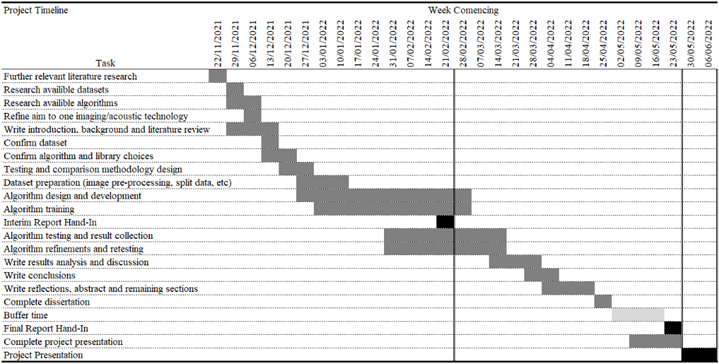
\includegraphics[width=\textwidth]{figures/gantt-chart.png}
    \caption{Project plan presented as a Gantt chart.}
    \label{fig:gantt-chart}
\end{figure}

\section{Software Development}


\section{Toolsets and Machine Environments}
Toolsets refer to both software development and to project management, so the coverage should address both. This section will outline the tools for software development and project management process; it will make appropriate comparisons between tools available and argue for the most appropriate selection based on metrics, possibly a matrix diagram and other criteria.

DO NOT justify the grounds for using specific toolsets and environments simply because you know them well or have developed skills already. 

\begin{itemize}
    \item python
    \item tensorflow
    \item keras
    \item tensorboard - visualisation? and hp tuning
    \item google cloud platform
    \item google colab
    \item sklearn - metrics and cv
\end{itemize}

\section{Research Methods}
You should investigate the types of research methods necessary to validly answer the research questions that your project addresses. You should cite relevant sources to justify your choices.
\begin{itemize}
    \item abductive
    \item primary data
    
\end{itemize}